\documentclass{beamer}
\usetheme{default}

\usepackage{hyperref}
\hypersetup{
	colorlinks=true,
	urlcolor=blue,
	linkcolor=magenta,
	citecolor=blue,
}

\usepackage{tikz}
\usepackage{tikz-cd}
\usepackage{mathtools}


%\theoremstyle{definition}
\renewcommand{\proofname}{Demostración}

\makeatletter
\newenvironment<>{proofs}[1][\proofname]{%
	\par
	\def\insertproofname{#1\@addpunct{.}}%
	\usebeamertemplate{proof begin}#2}
{\usebeamertemplate{proof end}}
\makeatother



\title{Chiral polytopes}
\author{Daniel González Casanova Azuela}

\begin{document}
\begin{frame}[plain]
    \maketitle
\end{frame}

\begin{frame}{History}
\begin{itemize}
\item Beginnings of interest in polygons and polyhedra is untracktable.

\item Euclid's Elements provide constructions of polygons and the five Platonic solids.

\item XIV century, an Archbishop of Canterbury investigated star polygons.

\item XVII century Kepler studied the two regular polyedra whose faces are pentagrams.

\end{itemize}	
\end{frame}

\begin{frame}
\begin{figure}[H]
	\centering
	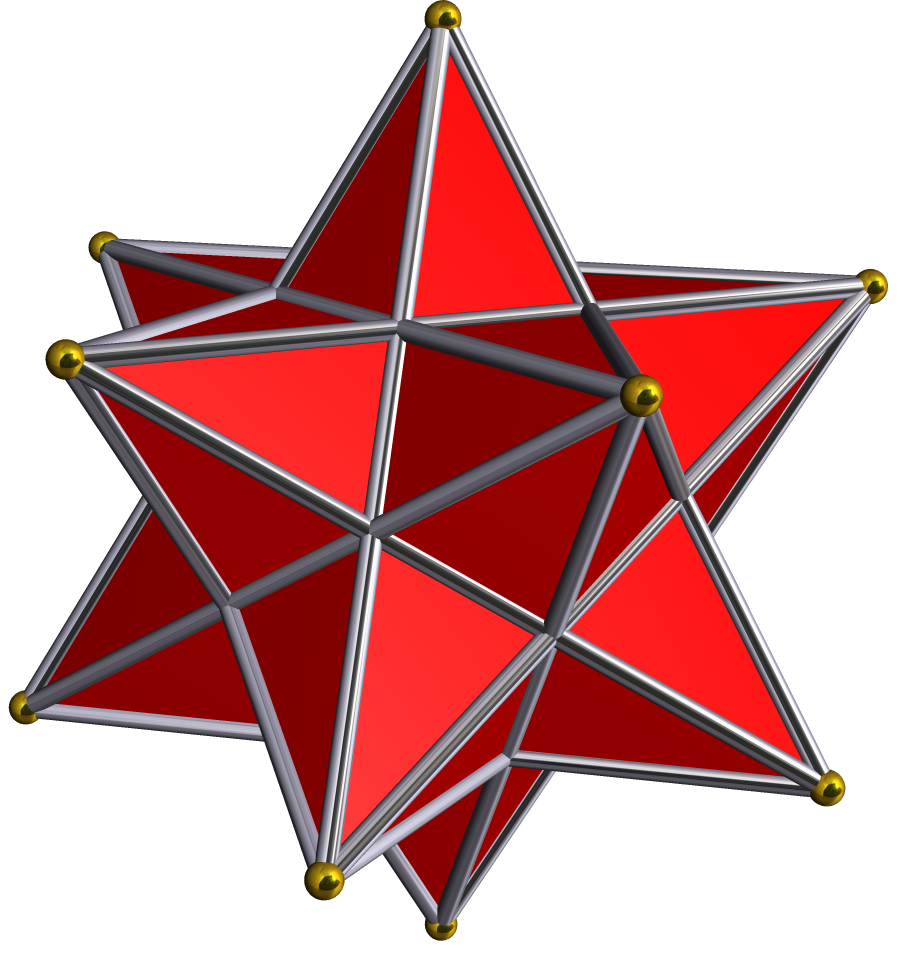
\includegraphics[width=0.5\textwidth]{fig1.png}
	\caption{Great stellated dodecahedron}
\end{figure}
\end{frame}

\begin{frame}
	\begin{itemize}
	\item 1809 Poinsot studied their duals: their faces are regular pentagons but their vertex-figures are pentagrams.

	\item XIX century Schl\"afli studied higher-dimensional polytopes.

	\item XX century Coxeter  classified all discrete euclidean reflection groups and several other results.

	\item 1930's Coxeter and Petrie admit infinite faces and find three more regular polyhedra in euclidean 3-space. They have non-planar vertex figures.

	\item 1977 Gr\"unbraum admits non-planar faces. There are 18 finite regular polyhedra and 48 in total.
	\end{itemize}
\end{frame}

\begin{frame}
	\begin{itemize}
	\item Around 1970 abstract polytopes are introduced as partial orders in different articles by McMullen, Gr\"unbraum.

	\item Chiral polytopes are introduced as abstract polytopes and later their realizations in euclidean space are studied (Schulte, Weiss).

	\item 2014 the first chiral 4-polytope in euclidean 4-space is introduced (Bracho, Hubard, Pellicer).

	\item In my master's thesis I used this construction to produce two chiral star 4-polytopes.
	\end{itemize}
\end{frame}

\begin{frame}{It's all the same!}
	\[\begin{tikzcd}[ampersand replacement=\&]
		\substack{\text{{\Large Geometry}}  \\ \text{Skeletal polytopes} } \arrow[rr]\arrow[dd]\&\&\substack{\text{{\Large Combinatorics}}\\\text{Abstract polytopes} }\arrow[ll]\arrow[dd]\\ \\
		\substack{\text{{\Large Group theory}}\\\text{Symmetry group} }\arrow[rr]\arrow[uu]\&\&\substack{\text{{\Large Group theory}}\\\text{Automorphism group} }\arrow[ll]\arrow[uu]
			\end{tikzcd}\]
\end{frame}

\begin{frame}{Axioms for abstract 4 polytopes}
	An \textit{\textbf{abstract polytope}} $\mathcal{P}$ is a partial order such that (\textit{\textbf{faces}}=elements of the poset,  \textit{\textbf{flags}}=chains).
	\begin{enumerate}
		\item $\mathcal{P}$ contains a minimal and a greatest face
	
		\item Flags include the 0 face and the top face.

		\item It is \textit{\textbf{strongly flag connected}}. (This implies connectedness in the geometric case)

		 \item \textit{\textbf{Diamond axiom}}. So that exactly two 2-faces are incident at each edge generalized.
	\end{enumerate}
\end{frame}

\begin{frame}{Regular and chiral abstract 4-polytopes}
\begin{itemize}
\item An \textit{\textbf{automorphism}} of $\mathcal{P}$ is a bijection that preserves incidence. These conform the group $\Gamma(\mathcal{P})$.
\item $\mathcal{P}$ is \textit{\textbf{regular}} if its automorphism group acts transitively on flags.
\item $\mathcal{P}$ is \textit{\textbf{chiral}} if $\Gamma(\mathcal{P})$ induces two orbits on flags and adjacent flags are in different orbits. (Rotation subgroup)
\end{itemize}
\end{frame}

\begin{frame}{Automorphism group of a regular abstract 4-polytope}
	Pick any flag and call it \textit{\textbf{base flag}}. There exist unique involutory automorphisms $\rho_j$ (these can be thought as reflections about the facets of a \textit{\textbf{base tetrahedron}}, which corresponds to the base flag) such that
	\begin{itemize}
		\item $(\rho_i\rho_j)^{p_{ij}}=\operatorname{id}$ when $|i-j| \geq 2$. The \textit{\textbf{Shl\"afli type}} of  $\mathcal{P}$ is $(p_1,p_2,p_3)$ (how many edges at a vertex, cells at an edge, etc.).
		\item \textit{\textbf{Intersection property}}.
	\end{itemize}
	A group satisfying these conditions yields an abstract polytope and vice-versa. Analogue conditions exist for the chiral case.
\end{frame}

\begin{frame}{Realizations of abstract 4-polytopes}
\begin{itemize}
\item A \textit{\textbf{realization}} of $\mathcal{P}$ is a map from the set of 0-faces into $\mathbb{R}^4$. This induces maps $\beta_i$ to faces of all dimensions.

\item A realization is \textit{\textbf{faithful}} if every $\beta_i$ is a bijection (the number of abstract faces coincides with geometric faces, no collapse).

\item A realization is \textit{\textbf{symmetric}} if every automorphism of $\mathcal{P}$ induces a permutation of the geometric faces, which in turn determine isometries of euclidean space.

\item Conversely, given an euclidean representation (a group of isometries isomorphic to the automorphism group) we may construct a geometric polytope taking copies of the base flag. This is called \textit{\textbf{Whythoff's construction}}.
\end{itemize}
\end{frame}

\begin{frame}{A chiral polytope in $\mathbb{R}^4$ }
\begin{itemize}
\item Bracho, Hubard, Pellicer found a skeletal chiral 4-polytope in $\mathbb{R}^4$ constructed from the 4-cube $\{4,3,3\}$ and determined the relations defining its symmetry group.

\item This construction led to a family of chiral polyhedra in $\mathbb{R}^4$, one of which is the cell of the former chiral 4-polytope.

\item I showed that two other of these chiral polyhedra may be used to construct chiral 4-polytopes. They are constructed from the star 4-polytopes $\left\{ \frac{5}{2},3,5 \right\} $ and its dual $\left\{ 5,3,\frac{5}{2} \right\} $.
\end{itemize}
\end{frame}

\begin{frame}
\begin{figure}[H]
	\centering
	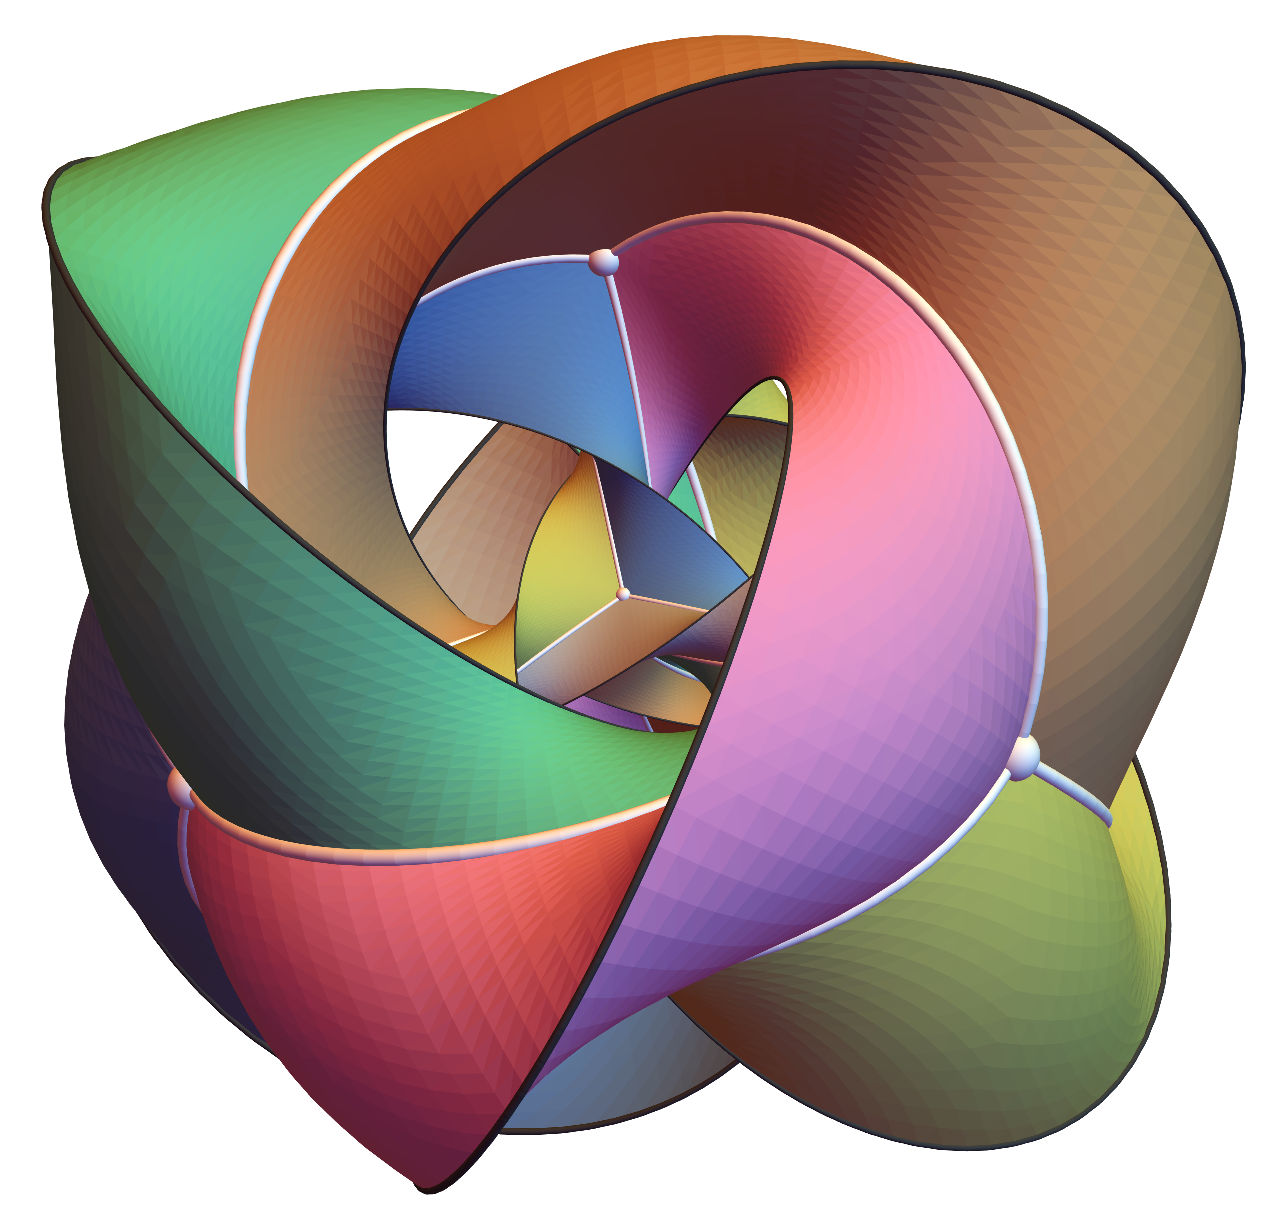
\includegraphics[width=0.5\textwidth]{fig2.png}
	\caption{Chiral dodecahedron}
\end{figure}
\end{frame}

\begin{frame}
\begin{figure}[H]
	\centering
	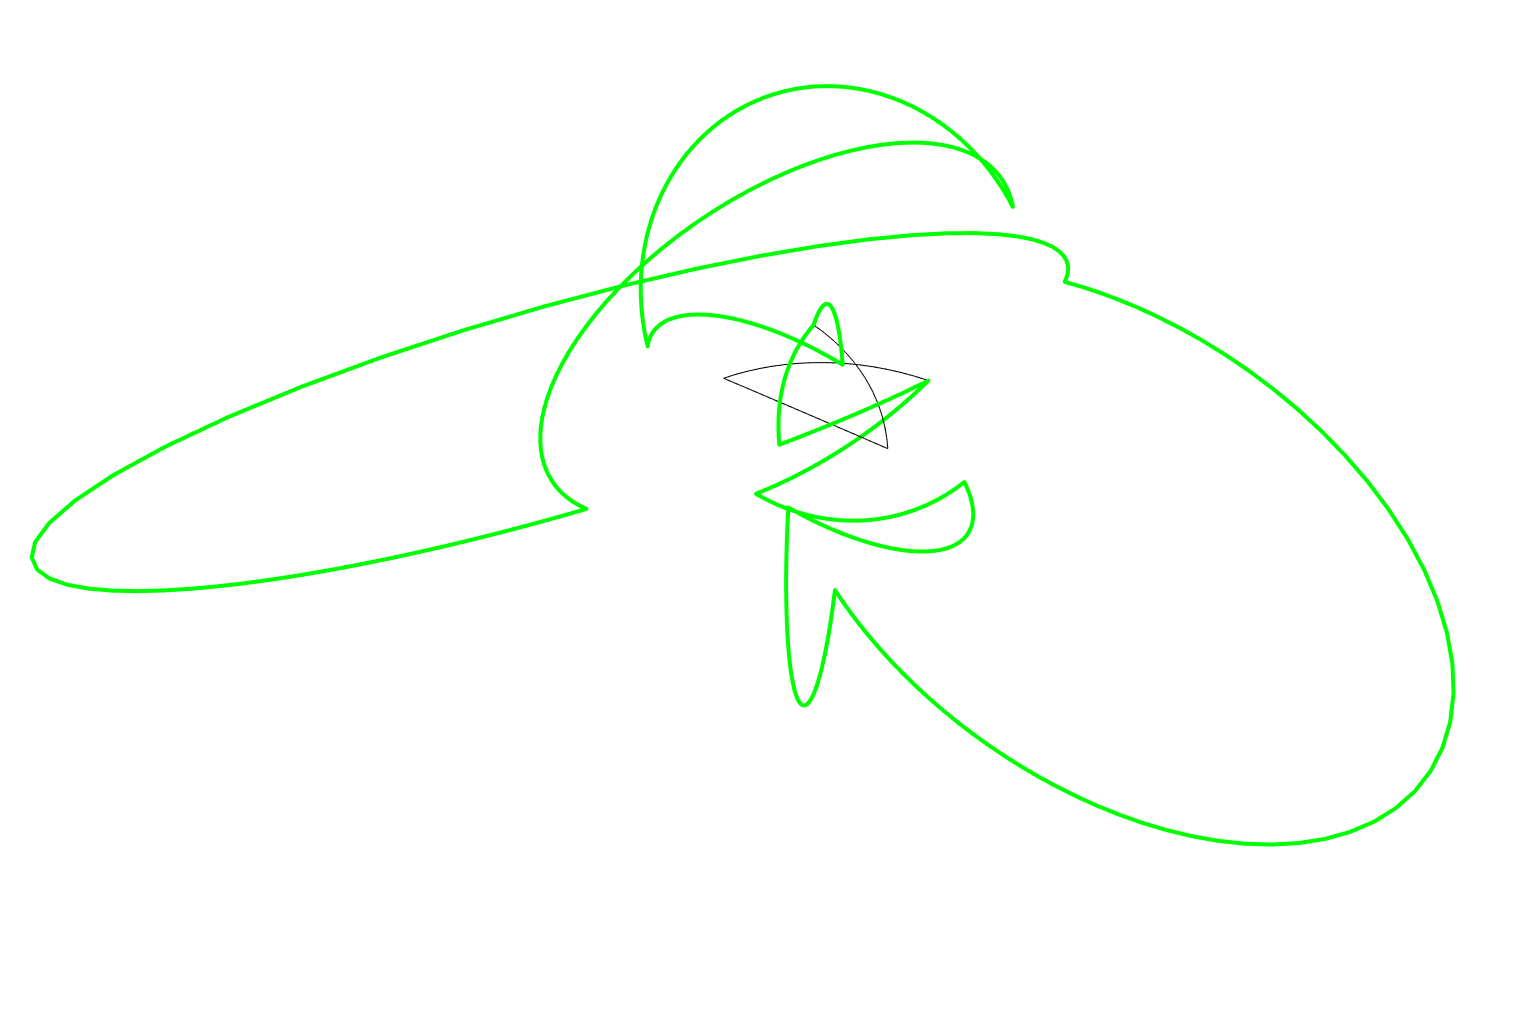
\includegraphics[width=0.5\textwidth]{fig3.png}
	\caption{A 2-face of my polytope}
\end{figure}
\end{frame}


\end{document}
